\begin{enumerate}[label=\thesection.\arabic*,ref=\thesection.\theenumi]
\numberwithin{equation}{enumi}
\numberwithin{figure}{enumi}
\numberwithin{table}{enumi}

\item 
\label{chapters/10/11/2/1}
	\\
	\solution See Fig. 
		\ref{fig:10/11/2/4}.
	\begin{figure}[!ht]
		\centering
 \includegraphics[width=\columnwidth]{chapters/10/11/2/4/figs/circle1.pdf}
		\caption{}
		\label{fig:10/11/2/4}
  	\end{figure}

\item 
\label{chapters/10/11/2/2}
	\\
	\solution See Fig. 
		\ref{fig:10/11/2/2}.
	\begin{figure}[H]
		\centering
 \includegraphics[width=0.75\columnwidth]{chapters/10/11/2/2/figs/main.png}
		\caption{}
		\label{fig:10/11/2/2}
  	\end{figure}


\item 
\label{chapters/10/11/2/3}
\\
\solution See Fig. 
		\ref{fig:10/11/2/3}.
	\begin{figure}[H]
		\centering
 \includegraphics[width=0.75\columnwidth]{chapters/10/11/2/3/figs/Question.png}
		\caption{}
		\label{fig:10/11/2/3}
  	\end{figure}

\item 
\label{chapters/10/11/2/4}
	\\
	\solution See Fig. 
		\ref{fig:10/11/2/4}.
	\begin{figure}[!ht]
		\centering
 \includegraphics[width=\columnwidth]{chapters/10/11/2/4/figs/circle1.pdf}
		\caption{}
		\label{fig:10/11/2/4}
  	\end{figure}

\item 
\label{chapters/10/11/2/5}
	\\
	\solution See Fig. 
		\ref{fig:10/11/2/4}.
	\begin{figure}[!ht]
		\centering
 \includegraphics[width=\columnwidth]{chapters/10/11/2/4/figs/circle1.pdf}
		\caption{}
		\label{fig:10/11/2/4}
  	\end{figure}

\item 
\label{chapters/10/11/2/6}
	\\
	\solution See Fig. 
		\ref{fig:10/11/2/4}.
	\begin{figure}[!ht]
		\centering
 \includegraphics[width=\columnwidth]{chapters/10/11/2/4/figs/circle1.pdf}
		\caption{}
		\label{fig:10/11/2/4}
  	\end{figure}

\item A tangent $PQ$ at a point of a circle of radius 5cm meets a line through the centre $O$ at a point $Q$ so that $OQ$=12cm then length of $PQ$ is
\label{chapters/10/10/1/3}
\\
\solution
	\begin{figure}[H]
		\centering
 \includegraphics[width=0.75\columnwidth]{chapters/12/6/3/8/figs/main.png}
		\caption{}
		\label{fig:12/6/3/8}
  	\end{figure}
The equation of the conic can be represented as
\begin{align}
\vec{x}^{\top}\myvec{1&0\\0&0}\vec{x}+2\myvec{-2&\frac{-1}{2}}\vec{x}+4=0
\end{align}
So,
\begin{align}
\vec{V}=\myvec{1&0\\0&0},
\vec{u}^{\top}=\myvec{-2&\frac{-1}{2}},
f=4
\end{align}
The direction vector of the line passing through (2,0) and (4,4) is 
\begin{align}
\vec{m}=\myvec{1\\2}
\implies
\vec{n}=\myvec{2\\-1}.
\end{align}
The eigenvector corresponding to the zero eigenvalue is 
\begin{align}
\vec{p}_1=\myvec{0\\1},
\end{align}
In
\eqref{eq:conic_tangent_q_eigen},
\begin{align}
	\kappa=\frac{\myvec{0&1}\myvec{-2\\ \frac{-1}{2}}}{\myvec{0&1}\myvec{2\\-1}}
	=\frac{1}{2}
\end{align}
Substituting  $\kappa$,
from 
\eqref{eq:conic_tangent_q_eigen},
\begin{align}
	\myvec{\sbrak{\myvec{-2\\\frac{-1}{2}}+\frac{1}{2}\myvec{2\\-1}}^{\top} \\ \myvec{1&0\\0&0}}\vec{q} &= \myvec{-4 \\ \frac{1}{2}\myvec{2\\-1}-\myvec{-2\\\frac{-1}{2}}}\\
	\implies
	\myvec{-1&-1 \\ 1&0 \\ 0&0}\vec{q}&=\myvec{-4 \\ 3 \\ 0}
\end{align}
yielding
\begin{align}
\myvec{-1&-1 \\ 1&0}\vec{q} = \myvec{-4\\3}
\end{align}
The augmented matrix is 
\begin{align*}
  \myvec{
                -1&-1&\vrule&-4\\
	        1&0&\vrule&3}
  \xleftrightarrow[]{R_1 \leftarrow R_1+ 2R_2}
     \myvec{
	         1&-1&\vrule&2\\
	         1&0&\vrule&3}
      \\
 \xleftrightarrow[]{R_2 \leftarrow R_2 - R_1}
     \myvec{
	         1&-1&\vrule&2\\
	         0&1&\vrule&1}
 \xleftrightarrow[]{R_1 \leftarrow R_1 + R_2}
     \myvec{
	         1&0&\vrule&3\\
	         0&1&\vrule&1}
      \\ \implies \vec{q}=\myvec{3\\1}
\end{align*}
which is the desired 
point of contact.
See Fig. 
		\ref{fig:12/6/3/8}.

\item 
\label{chapters/10/10/1/4}
	\\
	\solution See Fig. 
		\ref{fig:10/11/2/4}.
	\begin{figure}[!ht]
		\centering
 \includegraphics[width=\columnwidth]{chapters/10/11/2/4/figs/circle1.pdf}
		\caption{}
		\label{fig:10/11/2/4}
  	\end{figure}

\item From a point $\vec{Q}$, the length of the tangent to a circle is $24 cm$ and the distance of $\vec{Q}$ from the centre is $25 cm$. Find the radius of the circle. Draw the circle and the tangents. 
\label{chapters/10/10/2/1}
\\
\solution
	\begin{figure}[H]
		\centering
 \includegraphics[width=0.75\columnwidth]{chapters/12/6/3/8/figs/main.png}
		\caption{}
		\label{fig:12/6/3/8}
  	\end{figure}
The equation of the conic can be represented as
\begin{align}
\vec{x}^{\top}\myvec{1&0\\0&0}\vec{x}+2\myvec{-2&\frac{-1}{2}}\vec{x}+4=0
\end{align}
So,
\begin{align}
\vec{V}=\myvec{1&0\\0&0},
\vec{u}^{\top}=\myvec{-2&\frac{-1}{2}},
f=4
\end{align}
The direction vector of the line passing through (2,0) and (4,4) is 
\begin{align}
\vec{m}=\myvec{1\\2}
\implies
\vec{n}=\myvec{2\\-1}.
\end{align}
The eigenvector corresponding to the zero eigenvalue is 
\begin{align}
\vec{p}_1=\myvec{0\\1},
\end{align}
In
\eqref{eq:conic_tangent_q_eigen},
\begin{align}
	\kappa=\frac{\myvec{0&1}\myvec{-2\\ \frac{-1}{2}}}{\myvec{0&1}\myvec{2\\-1}}
	=\frac{1}{2}
\end{align}
Substituting  $\kappa$,
from 
\eqref{eq:conic_tangent_q_eigen},
\begin{align}
	\myvec{\sbrak{\myvec{-2\\\frac{-1}{2}}+\frac{1}{2}\myvec{2\\-1}}^{\top} \\ \myvec{1&0\\0&0}}\vec{q} &= \myvec{-4 \\ \frac{1}{2}\myvec{2\\-1}-\myvec{-2\\\frac{-1}{2}}}\\
	\implies
	\myvec{-1&-1 \\ 1&0 \\ 0&0}\vec{q}&=\myvec{-4 \\ 3 \\ 0}
\end{align}
yielding
\begin{align}
\myvec{-1&-1 \\ 1&0}\vec{q} = \myvec{-4\\3}
\end{align}
The augmented matrix is 
\begin{align*}
  \myvec{
                -1&-1&\vrule&-4\\
	        1&0&\vrule&3}
  \xleftrightarrow[]{R_1 \leftarrow R_1+ 2R_2}
     \myvec{
	         1&-1&\vrule&2\\
	         1&0&\vrule&3}
      \\
 \xleftrightarrow[]{R_2 \leftarrow R_2 - R_1}
     \myvec{
	         1&-1&\vrule&2\\
	         0&1&\vrule&1}
 \xleftrightarrow[]{R_1 \leftarrow R_1 + R_2}
     \myvec{
	         1&0&\vrule&3\\
	         0&1&\vrule&1}
      \\ \implies \vec{q}=\myvec{3\\1}
\end{align*}
which is the desired 
point of contact.
See Fig. 
		\ref{fig:12/6/3/8}.

\item In Fig. \ref{fig:chapters/10/10/2/2/Fig1}, if TP and TQ are two tangents to a circle with centre O so that $\angle{POQ} = 110\degree$ then find $\angle{PTQ}$. 
\\
\solution
	\begin{figure}[H]
		\centering
 \includegraphics[width=0.75\columnwidth]{chapters/12/6/3/8/figs/main.png}
		\caption{}
		\label{fig:12/6/3/8}
  	\end{figure}
The equation of the conic can be represented as
\begin{align}
\vec{x}^{\top}\myvec{1&0\\0&0}\vec{x}+2\myvec{-2&\frac{-1}{2}}\vec{x}+4=0
\end{align}
So,
\begin{align}
\vec{V}=\myvec{1&0\\0&0},
\vec{u}^{\top}=\myvec{-2&\frac{-1}{2}},
f=4
\end{align}
The direction vector of the line passing through (2,0) and (4,4) is 
\begin{align}
\vec{m}=\myvec{1\\2}
\implies
\vec{n}=\myvec{2\\-1}.
\end{align}
The eigenvector corresponding to the zero eigenvalue is 
\begin{align}
\vec{p}_1=\myvec{0\\1},
\end{align}
In
\eqref{eq:conic_tangent_q_eigen},
\begin{align}
	\kappa=\frac{\myvec{0&1}\myvec{-2\\ \frac{-1}{2}}}{\myvec{0&1}\myvec{2\\-1}}
	=\frac{1}{2}
\end{align}
Substituting  $\kappa$,
from 
\eqref{eq:conic_tangent_q_eigen},
\begin{align}
	\myvec{\sbrak{\myvec{-2\\\frac{-1}{2}}+\frac{1}{2}\myvec{2\\-1}}^{\top} \\ \myvec{1&0\\0&0}}\vec{q} &= \myvec{-4 \\ \frac{1}{2}\myvec{2\\-1}-\myvec{-2\\\frac{-1}{2}}}\\
	\implies
	\myvec{-1&-1 \\ 1&0 \\ 0&0}\vec{q}&=\myvec{-4 \\ 3 \\ 0}
\end{align}
yielding
\begin{align}
\myvec{-1&-1 \\ 1&0}\vec{q} = \myvec{-4\\3}
\end{align}
The augmented matrix is 
\begin{align*}
  \myvec{
                -1&-1&\vrule&-4\\
	        1&0&\vrule&3}
  \xleftrightarrow[]{R_1 \leftarrow R_1+ 2R_2}
     \myvec{
	         1&-1&\vrule&2\\
	         1&0&\vrule&3}
      \\
 \xleftrightarrow[]{R_2 \leftarrow R_2 - R_1}
     \myvec{
	         1&-1&\vrule&2\\
	         0&1&\vrule&1}
 \xleftrightarrow[]{R_1 \leftarrow R_1 + R_2}
     \myvec{
	         1&0&\vrule&3\\
	         0&1&\vrule&1}
      \\ \implies \vec{q}=\myvec{3\\1}
\end{align*}
which is the desired 
point of contact.
See Fig. 
		\ref{fig:12/6/3/8}.

\item If the tangents $PA$ and $PB$ from a point $\vec{P}$ to a circle with center $\vec{O}$ are inclined to each other at $80{\degree}$, find $\angle{POA}$.
\\
\solution
	\begin{figure}[H]
		\centering
 \includegraphics[width=0.75\columnwidth]{chapters/12/6/3/8/figs/main.png}
		\caption{}
		\label{fig:12/6/3/8}
  	\end{figure}
The equation of the conic can be represented as
\begin{align}
\vec{x}^{\top}\myvec{1&0\\0&0}\vec{x}+2\myvec{-2&\frac{-1}{2}}\vec{x}+4=0
\end{align}
So,
\begin{align}
\vec{V}=\myvec{1&0\\0&0},
\vec{u}^{\top}=\myvec{-2&\frac{-1}{2}},
f=4
\end{align}
The direction vector of the line passing through (2,0) and (4,4) is 
\begin{align}
\vec{m}=\myvec{1\\2}
\implies
\vec{n}=\myvec{2\\-1}.
\end{align}
The eigenvector corresponding to the zero eigenvalue is 
\begin{align}
\vec{p}_1=\myvec{0\\1},
\end{align}
In
\eqref{eq:conic_tangent_q_eigen},
\begin{align}
	\kappa=\frac{\myvec{0&1}\myvec{-2\\ \frac{-1}{2}}}{\myvec{0&1}\myvec{2\\-1}}
	=\frac{1}{2}
\end{align}
Substituting  $\kappa$,
from 
\eqref{eq:conic_tangent_q_eigen},
\begin{align}
	\myvec{\sbrak{\myvec{-2\\\frac{-1}{2}}+\frac{1}{2}\myvec{2\\-1}}^{\top} \\ \myvec{1&0\\0&0}}\vec{q} &= \myvec{-4 \\ \frac{1}{2}\myvec{2\\-1}-\myvec{-2\\\frac{-1}{2}}}\\
	\implies
	\myvec{-1&-1 \\ 1&0 \\ 0&0}\vec{q}&=\myvec{-4 \\ 3 \\ 0}
\end{align}
yielding
\begin{align}
\myvec{-1&-1 \\ 1&0}\vec{q} = \myvec{-4\\3}
\end{align}
The augmented matrix is 
\begin{align*}
  \myvec{
                -1&-1&\vrule&-4\\
	        1&0&\vrule&3}
  \xleftrightarrow[]{R_1 \leftarrow R_1+ 2R_2}
     \myvec{
	         1&-1&\vrule&2\\
	         1&0&\vrule&3}
      \\
 \xleftrightarrow[]{R_2 \leftarrow R_2 - R_1}
     \myvec{
	         1&-1&\vrule&2\\
	         0&1&\vrule&1}
 \xleftrightarrow[]{R_1 \leftarrow R_1 + R_2}
     \myvec{
	         1&0&\vrule&3\\
	         0&1&\vrule&1}
      \\ \implies \vec{q}=\myvec{3\\1}
\end{align*}
which is the desired 
point of contact.
See Fig. 
		\ref{fig:12/6/3/8}.

\item 
\label{chapters/10/10/2/4}
	\\
	\solution See Fig. 
		\ref{fig:10/11/2/4}.
	\begin{figure}[!ht]
		\centering
 \includegraphics[width=\columnwidth]{chapters/10/11/2/4/figs/circle1.pdf}
		\caption{}
		\label{fig:10/11/2/4}
  	\end{figure}

\item 
\label{chapters/10/10/2/5}
%	\\
	\solution See Fig. 
		\ref{fig:10/11/2/4}.
	\begin{figure}[!ht]
		\centering
 \includegraphics[width=\columnwidth]{chapters/10/11/2/4/figs/circle1.pdf}
		\caption{}
		\label{fig:10/11/2/4}
  	\end{figure}

\item 
\label{chapters/10/10/2/6}
	\\
	\solution See Fig. 
		\ref{fig:10/11/2/4}.
	\begin{figure}[!ht]
		\centering
 \includegraphics[width=\columnwidth]{chapters/10/11/2/4/figs/circle1.pdf}
		\caption{}
		\label{fig:10/11/2/4}
  	\end{figure}

\item 
\label{chapters/10/10/2/7}
	\\
	\solution See Fig. 
		\ref{fig:10/11/2/4}.
	\begin{figure}[!ht]
		\centering
 \includegraphics[width=\columnwidth]{chapters/10/11/2/4/figs/circle1.pdf}
		\caption{}
		\label{fig:10/11/2/4}
  	\end{figure}

\item 
\label{chapters/10/10/2/8}
	\\
	\solution See Fig. 
		\ref{fig:10/11/2/4}.
	\begin{figure}[!ht]
		\centering
 \includegraphics[width=\columnwidth]{chapters/10/11/2/4/figs/circle1.pdf}
		\caption{}
		\label{fig:10/11/2/4}
  	\end{figure}

\item 
\label{chapters/10/10/2/9}
	\\
	\solution See Fig. 
		\ref{fig:10/11/2/4}.
	\begin{figure}[!ht]
		\centering
 \includegraphics[width=\columnwidth]{chapters/10/11/2/4/figs/circle1.pdf}
		\caption{}
		\label{fig:10/11/2/4}
  	\end{figure}

\item 
\label{chapters/10/10/2/10}
	\\
	\solution See Fig. 
		\ref{fig:10/11/2/4}.
	\begin{figure}[!ht]
		\centering
 \includegraphics[width=\columnwidth]{chapters/10/11/2/4/figs/circle1.pdf}
		\caption{}
		\label{fig:10/11/2/4}
  	\end{figure}

\item 
%\label{chapters/10/10/2/10}
%	\\
	\solution See Fig. 
		\ref{fig:10/11/2/4}.
	\begin{figure}[!ht]
		\centering
 \includegraphics[width=\columnwidth]{chapters/10/11/2/4/figs/circle1.pdf}
		\caption{}
		\label{fig:10/11/2/4}
  	\end{figure}

\item 
\label{chapters/10/10/2/12}
	\\
	\solution See Fig. 
		\ref{fig:10/11/2/4}.
	\begin{figure}[!ht]
		\centering
 \includegraphics[width=\columnwidth]{chapters/10/11/2/4/figs/circle1.pdf}
		\caption{}
		\label{fig:10/11/2/4}
  	\end{figure}

 \item Prove that opposite sides of a quadrilateral circumscribing a circle 
    subtend supplementary angles at the centre of the circle.
\label{chapters/10/10/2/13}
\\
       \solution 
	\\
	\solution See Fig. 
		\ref{fig:10/11/2/4}.
	\begin{figure}[!ht]
		\centering
 \includegraphics[width=\columnwidth]{chapters/10/11/2/4/figs/circle1.pdf}
		\caption{}
		\label{fig:10/11/2/4}
  	\end{figure}

\item Find the equation of a circle whose centre is (3,1) and which cuts off a chord of length  6 units on the  line 2x-5y+18=0
\item Find the equation of a circle of redius 5 which is touching another circle $x^2+y^2-2x-4y-20=0$ at (5,5).
Fill in the Blanks
\begin{enumerate}[label=\thesection.\arabic*,ref=\thesection.\theenumi,resume*]
\item The equation of the circle having centre at (3,-4) and touching the line $5x+12y-12=0$ is \makebox[1cm]{\hrulefill}                     
\item The equation of the circle circumscribing the triangle whose sides are the lines $y=x+2, 3y=4x, 2y=3x$ is  \makebox[1cm]{\hrulefill}         

\end{enumerate}
